\section{Lebesgue Measure} 

  We have seen that there are some common sets that are not Jordan measurable, but a bigger problem is that countable unions and intersections aren't. 

  \begin{example}[Countable Union/Intersection of Jordan Measurable Sets are Not J.M.]
    We show a few counterexamples. 
    \begin{enumerate}
      \item \textit{Countable Union}. Take $\mathbb{N} = \{n\}_{n=1}^\infty$. Each point $n$ has Jordan measure $0$, but their union is unbounded so it isn't Jordan measurable. 

      \item \textit{Bounded Countable Union}. Maybe we can fix this by considering bounded unions. But consider $E = \mathbb{Q} \cap [0, 1]$. By density of rationals, 
      \begin{equation}
        m_\ast (E) = 0 \neq 1 = m^\ast (E)
      \end{equation}
        
      \item \textit{Intersection}. Consider the Cantor set $C$, which is bounded, but again 
      \begin{equation}
        m_\ast (C) = 0 \neq 1 = m^\ast (C)
      \end{equation}
    \end{enumerate}
  \end{example}

  In some applications, we can just ignore some of these sets as ``pathological.'' But for Riemann integrability, we are integrating over Jordan measurable sets. I turns out that it is really important that we can \textit{at least} guarantee that countable unions and intersections of Jordan measurable sets are measurable. If we don't, then not even uniform convergence---an extremely strong property---can preserve continuity, differentiability, and integrability of a sequence of functions. 

  \begin{example}[Disasters of Uniform Limit of Integrable Functions is Not Integrable]
    Tao Exercise 1.2.2. 
  \end{example}

  This motivates the definition of a $\sigma$-algebra. 

  \begin{definition}[$\sigma$-Algebra]
    A \textbf{$\boldsymbol{\sigma}$-algebra} on a set $X$ is a collection of subsets of $X$ satisfying the following: 
    \begin{enumerate}
      \item \textit{Contains Empty and Full Set}. $\emptyset, X \in \mathcal{A}$. 
      \item \textit{Closed Under Countable Unions}. $A_n \in \mathcal{A}$ for all $n \in \mathbb{N}$ implies $\bigcup_n A_n \in \mathcal{A}$. 
      \item \textit{Closed Under Complements}. $A \in \mathcal{A} \implies A^c \in \mathcal{A}$. 
      \item \textit{Closed Under Countable Intersections}.\footnote{This is actually a consequence of the previous properties. We can utilize the fact that $\cap_{k=1}^\infty A_k = X \setminus \cup_{k=1}^\infty A_k^c$ } $A_n \in \mathcal{A}$ for all $n \in \mathbb{N}$ implies $\bigcap_n A_n \in \mathcal{A}$. 
    \end{enumerate}
  \end{definition}

\subsection{Lebesgue Outer Measure}

  Therefore, we would like the collection of our measurable sets to be a $\sigma$-algebra. To do this, we tinker around with the definition of the Jordan measure. Note that by definition, the Jordan outer measure can be equivalently written as 
  \begin{align}
    m^\ast (S) & \coloneqq \inf \{ m(E) \mid S \subset E, E \text{ elementary} \} \\ 
               & = \inf \bigg\{ \sum_{i=1}^k |B_i| \;\bigg|\; S \subset \bigcup_{i=1}^k B_i, B_i \text{ boxes}, k \in \mathbb{N} \bigg\}
  \end{align}
  Note that the \textit{finite} number of boxes $k$ are allowed to vary over all naturals. To define the Lebesgue measure, we change the finite to countable.

  \begin{definition}[Lebesgue Outer Measure]
    Given any set $E \subset \mathbb{R}^n$, the \textbf{Lebesgue outer measure} is a map 
    \begin{equation}
      m^\ast : 2^{\mathbb{R}^n} \to [0, +\infty], \qquad m^\ast (E) = \inf  \left\{ \sum_{k=1}^\infty |B_k| \; \bigg| \; E \subset \bigcup_{k=1}^\infty B_k \right\} 
    \end{equation}
  \end{definition} 

  It's a hard definition, but a natural one, since we're taking all these boxes and trying to make them as snug as possible to define the outer measure of an arbitrary set. We first first check that this is indeed a generalization of Jordan measure, in the sense that if $E$ is Jordan measurable, then its Lebesgue outer measure is the same as its Jordan measure. 

  \begin{theorem}[Lebesgue Outer Measure Coincides with Interval Length]
    $m^\ast$ satisfies the property that for any interval $I \subset \mathbb{R}$, $m^\ast (I) = |I|$. 
  \end{theorem}
  \begin{proof}
    Let's first consider the case when $I$ is closed. Let $I = [a, b]$. Then, we know from definition that 
    \begin{equation}
      m^\ast (I) \coloneqq \inf \bigg\{ \sum_{k=1}^\infty |I_k| \;\bigg|\; I \subset \bigcup_{k=1}^\infty I_k\bigg\}
    \end{equation}
    where $I_k = [a_n, b_n]$. We wish to show that the above quantity equals $b - a$. 
    \begin{enumerate}
      \item $m^\ast (I) \leq b - a$. This is pretty easy since we can just set the cover to consist of the single interval $I$, and since $m^\ast (I)$ must be the infimum of it, then we must have $m^\ast(I) \leq b - a$. A technicality is that we must strictly use countable covers, but in this case, we can just fix $\epsilon > 0$ and see 
      \begin{equation}
        I_1 = [a, b], \qquad I_k = [b - \frac{\epsilon}{2^k}, b + \frac{\epsilon}{2^k}]
      \end{equation}
      In this case the sums of lengths of all $I_2, \ldots$ is $\epsilon/2 < \epsilon$, and so 
      \begin{equation}
        I_k \leq b - a + \epsilon \qquad \forall \epsilon > 0 
      \end{equation}

      \item Proving $m^\ast (I) \geq b - a$ is harder. In here, we use the ``$\epsilon$ of room'' trick. Take any $\epsilon > 0$. Then there exists a cover $\{I_k\}_k$ s.t. 
      \begin{equation}
        m^\ast(I) = \epsilon \geq \sum_{k=1}^\infty |I_k| = \sum_{k=1}^\infty b_k - a_k
      \end{equation}
      All we wish to show that the RHS $\geq b - a$, but we can't really manipulate the infinite sum. This is where we use the fact that $[a, b]$ is compact\footnote{since it's closed and bounded}, and so we can take a finite subcover $\{I_{k_j}\}_{j=1}^n$. Therefore, 
      \begin{equation}
        m^\ast (I) + \epsilon  \geq \sum_{j=1}^n b_{k_j} - a_{k_j} 
      \end{equation}
      Now we can rearrange this: set the $a_{k_j}$'s to be increasing, and for simplicity let's reindex them to $a_j, b_j$. Then, it must be the case that $a_1 < a$. 
      \begin{enumerate}
        \item Consider $(a_1, b_1)$. If $b_1 > b$, we are done. 
        \item Otherwise, $b_1 \in (a_2, b_2)$. If $b_2 > b$, then 
        \begin{equation}
          b_2 - a_2 + b_1 - a_1 \geq b_2 - a_1 > b - a
        \end{equation}
        \item If not, then we keep going until we get to $(a_n, b_n)$. If $b_n > b$, then 
          \begin{equation}
            b_n - a_n + b_{n-1} - a_{n-1} + \ldots + b_1 - a_1 \geq b_n - a_1  > b - a
          \end{equation}
      \end{enumerate}
    \end{enumerate}
  \end{proof}

  The proof may be a bit unfamiliar since we have used two tricks. 
  \begin{enumerate}
    \item \textit{Geometric Sequence of $\epsilon$ Trick}. To account for countable collections, we set $\epsilon$ to be decreasing geometrically so that the series converges to $\epsilon$. 
    \begin{equation}
      \epsilon = \sum_{n=1}^\infty \frac{\epsilon}{2^n}
    \end{equation}

    \item \textit{$\epsilon$ of Room Trick}. This trick is used often when you need an opposite inequality that isn't as obvious, and it can only be used for inequalities involving a supremum or infimum. 
    \begin{equation}
      \inf\{S\} \geq x
    \end{equation}

    By using the definition of sup/inf as the \textit{least} upper/lower bound, we can scooch over by an $\epsilon$ to find an element in $s \in S$ that does satisfy the inequality 
    \begin{equation}
      \inf\{S\} + \epsilon > s \geq x
    \end{equation}
    and since $\epsilon$ was arbitrary, we are done. 
  \end{enumerate}

  It is clear that the Lebesgue outer measure is always less than the Jordan outer measure. 
  \begin{equation}
    m^\ast (E) \leq m^{(J), \ast} (E) 
  \end{equation}
  When are these different? 

  \begin{example}[Lebesgue Outer Measure Much Smaller than Jordan Outer Measure]
    Consider $\mathbb{Q}$. 
    \begin{enumerate}
      \item The Jordan outer measure is $+\infty$ since it is unbounded. 
      \item However, any countable set of $\mathbb{R}$ has Lebesgue outer measure $0$. Just enumerate $E = \{x_1, \ldots \}$. Then, we set $I_k = \big( x_k - \frac{\epsilon}{2^k}, x_k + \frac{\epsilon}{2^k} \big)$. Then, 
      \begin{equation}
        \sum_{k=1}^\infty \ell(I_k) = \epsilon
      \end{equation}
    \end{enumerate}
  \end{example}

  What about the inner measure? It turns out that we don't get much if we replace the finite to countable in the Jordan inner measure. 

  \begin{lemma}[Axiomatic Properties of Lebesgue Outer Measure]
    The Lebesgue outer measure satisfies the following. 
    \begin{enumerate}
      \item \textit{Null Empty Set}. $m^\ast(\emptyset) = 0$. 
      \item \textit{Monotonicity}. Given sets $E \subset F \subset \mathbb{R}^n$, we have 
      \begin{equation}
        m^\ast (E) \leq m^\ast (F)
      \end{equation}
    \item \textit{Countable Subadditivity}. For any countable collection of subsets $\{E_k\}$ of $\mathbb{R}^d$, 
      \begin{equation}
        m^\ast \bigg( \bigcup_n E_n \bigg) \leq \sum_{n} m^\ast (E_n) 
      \end{equation}
    \end{enumerate}
  \end{lemma}
  \begin{proof}
    The first two properties are trivial. For the third, let's start by writing out the definition for the outer measure for each $E_n$. 
    \begin{equation}
      m^\ast (E_n) \coloneqq \inf \bigg\{ \sum_{k=1}^\infty |B_k^{(n)}| \;\bigg|\; E_n \subset \bigcup_{k=1}^\infty B_k^{(n)}, B_k^{(n)} \text{ boxes} \bigg\}
    \end{equation}
    Somehow, we want to sum these values over all $n$ and prove that this is greater than the measure of the union. The first realization should be that for a fixed cover $\{B_k^{(n)}\}_k$ of $E_n$, the collection 
    \begin{equation}
      \{B_k^{(n)}\}_{n, k} \text{ covers } \bigcup_{n} E_n
    \end{equation} 
    This gives us a clue as to comparing the collection of covers of each $E_n$, with the cover of $\cup E_n$. There is no straightforward way to do this,\footnote{On one side, we have the sum of a countable number of infimums of some sets, and on the other hand, we have the infimum of the unions of all of these sets.} so we want to try and \textit{fix} these collections. We can do this with the $\epsilon$ of room trick. For each $E_n$, we can find a cover $\{B_k^{(n)}\}_k$ s.t. 
    \begin{equation}
      m^\ast (E_n) + \frac{\epsilon}{2^n} \geq \sum_{k=1}^\infty |B_k^{(n)}| 
    \end{equation}
    Then, we can take the infinite sum. 
    \begin{equation}
      \sum_{n=1}^\infty \bigg( m^\ast (E_n) + \frac{\epsilon}{2^n} \bigg) \geq \sum_{n=1}^\infty \sum_{k=1}^\infty |B_k^{(n)}| \geq m^\ast \bigg( \bigcup_n E_n \bigg)
    \end{equation} 
    where the final inequality follows from the fact that $\{B_k^{(n)}\}_{n, k}$ is a cover of $\cup_n E_n$, and so it must be greater than the infimum of all possible covers. All monotonic series converge in $[0, +\infty]$, so we can ``take out'' the $\epsilon$ term to get 
    \begin{equation}
      \epsilon + \sum_{n=1}^\infty m^\ast (E_n) \geq m^\ast \bigg( \bigcup_n E_n \bigg)
    \end{equation}
    which holds for all $\epsilon > 0$, and so we are done. 
  \end{proof}

  \begin{theorem}[Translation Invariance]
    $m^\ast$ is translation invariant. That is, for any $E \subset \mathbb{R}^n$, 
    \begin{equation}
      m^\ast (E) = m^\ast (E + a), \qquad E + a \coloneqq \{x + a \in \mathbb{R}^n \mid a \in E \}
    \end{equation}
  \end{theorem}
  \begin{proof}
    This is straightforward and requires no tricks. Note that 
    \begin{equation}
      \{B_k\} \text{ is a countable cover of } E \iff \{B_k + a\} \text{ is a countable cover of } E + a
    \end{equation}
    It is also clear that 
    \begin{equation}
      |B| = |B + a| 
    \end{equation}
    for any box $B \subset \mathbb{R}^n$, so the sets of sizes that we are taking the infimum over is exactly the same between the two. 
  \end{proof}

  The final property claims that we can always drop an outer-measure $0$ set and it won't affect the outer measure of the original set. Therefore, when talking about measurability of intervals, we don't have to worry about endpoints, or even whether it is missing a countable number of elements from it! 

  \begin{lemma}[Sets of Measure 0 have no Effect]
    Suppose $m^\ast (E) = 0$ and $A$ is any set. Then, $m^\ast (A \cup E) = m^\ast (A)$. 
  \end{lemma}
  \begin{proof}
    We have 
    \begin{equation}
      m^\ast (A \cup E) = \underbrace{m^\ast \big( (A \cup E) \cap E \big)}_{=0} + m^\ast \underbrace{\big( (A \cup E) \cap E^c \big)}_{\subset A} \leq m^\ast (A) \leq m^\ast (A)
    \end{equation}
    But $A \cup E \supset A$, so $m^\ast (A \cup E) = m^\ast (A)$. 
  \end{proof}

\subsection{Measurable Sets}

  The next step is to take the outer measure and define \textit{Lebesgue measurable} sets. The problem is that---unlike the Jordan measure---we don't have the inner measure to work with. This turns out to be not much of a problem, since through \textit{Littlewood's first principle}\footnote{One of the major themes in measure theory, where we say that measurable sets are well-approximated by open and closed sets.}, we can define measurability as being well-approximated by an open set. 
  
  \begin{definition}[Measurable Set]
    A set $E \subset \mathbb{R}^d$ is \textbf{Lebesgue measurable} if it satisfies one of the equivalent properties. 
    \begin{enumerate}
      \item \textit{Carathéodory's criterion}.\footnote{Colloquially, no matter how nasty a subset $A$ is, $E$ should be nice enough that we can cut $E$ into two pieces $C$ and $D$.} For every set $A \subset \mathbb{R}^n$, 
      \begin{equation}
        m^\ast (A) = m^\ast (A \cap E) + m^\ast (A \cap E^c)
      \end{equation}
      Note that due to countable subadditivity, we are guaranteed to have $\leq$. Therefore, it suffices to prove only for $\geq$. The sets with which this inequality is strict is not measurable, and the measurable sets specifically satisfy equality for countable sets.

      \item \textit{Outer Approximately Open}. $\forall \epsilon > 0$, $\exists$ open set $O \supset E$  s.t. $m(O \setminus E) \leq \epsilon$. 

      \item \textit{Inner Approximately Closed}. $\forall \epsilon > 0$, $\exists$ closed set $F \subset E$ s.t. $m^\ast (E \setminus F) < \epsilon$.  

      \item \textit{Outer Exactly $G_\delta$}. $\exists$ a $G_\delta$ set $G$ s.t. $E \subset G$ and $m^\ast (G \setminus E) = 0$. 

      \item \textit{Inner Exactly $F_\sigma$}. $\exists$ a $F_\sigma$ set $F$ s.t. $F \subset E$ and $m^\ast (E \setminus F) = 0$. 
    \end{enumerate}
  \end{definition}
  \begin{proof}
    Listed. 
    \begin{enumerate}
      \item (2) $\implies$ (1). Then for every $k \in \mathbb{N}$, we can find $O_k \supset E$ s.t. $m^\ast (O_k \setminus E) \leq 1/k$. Define the $G_\delta$ set $G = \cap_{k=1}^\infty O_k$. Then, $(G \setminus E) \subset (O_k \setminus E)$ for all $k \implies m^\ast (G \setminus E) \leq 1/k$ for all $k$. Therefore $m^\ast (G \setminus E) = 0$, and $E = G \setminus (G \setminus E)$ is measurable. 

      \item (1) $\implies$ (2). Assume $m^\ast (E) < +\infty$. Find a cover $\{I_k \}_{k=1}^\infty$ s.t. $\sum_{k=1}^\infty \ell (I_k) \leq m^\ast (E) + \epsilon$ . Call $O = \cup_k I_k$. Since $E$ is measurable, $m^\ast (O \setminus E) = m^\ast (O) - m^\ast (E) \leq \sum_{k=1}^\infty \ell(I_k) - m^\ast (E) \leq \epsilon$ 

      \item (1) $\iff$ (3). Straightforward with argument above.  

      \item (1) $\iff$ (4). Generally, we use the fact that $E$ measurable iff $E^c$ measurable. Find $O \supset E^c$ open, with $m^\ast (O \setminus E^c) \leq \epsilon$. Then $F = O^c$ is closed, $F \subset E$, and $m^\ast (E \setminus F) \leq \epsilon$. 

      \item (1) $\iff$ (5). Same argument as (1) $\iff$ (4). 
    \end{enumerate}
  \end{proof}

  Depending on the context, it is helpful to use one definition over another when proving measurability. Just remember that the Carathéodory definition is the most general, since it doesn't even assume a topology on a space, and that is the definition that we will use by default. So what kind of sets are measurable? 

  \begin{example}[Outer Measure $0$ Sets are Lebesgue Measurable]
    For any outer measure $m^\ast$ on $X$, $E \subset X$ with $m^\ast (E) = 0$  implies that $E$ is $m^\ast$-measurable. Take any $A$. Then $(A \cap E) \subset E$ and $(A \cap E^c) \subset A$. So by monotonicity, 
    \begin{equation}
      m^\ast(A \cap E) + m^\ast (A \cap E^c) \leq m^\ast(E) + m^\ast(A) = m^\ast (A)
    \end{equation}
    and this by definition means that $E$ is measurable. 
  \end{example}

  We could continue with more examples, but our main priority is to show that this family of Lebesgue measurable sets is indeed a $\sigma$-algebra, and it covers much more than Jordan measurable sets. The path to prove that countable unions are measurable is a long one, and we'll a lot of lemmas. 

  \begin{lemma}[Complements of Measurable Sets are Measurable]
    If $E$ is measurable, then so is $E^c$. 
  \end{lemma}
  \begin{proof}
    The definition is symmetric in both $E$ and $E^c$. 
  \end{proof}

  \begin{lemma}[Excision Property]
    If $E \subset \mathbb{R}^n$ is measurable with $m^\ast (E) < +\infty$, and $E \subset F$ for arbitrary set $F$, then 
    \begin{equation}
      m^\ast (F \setminus E) = m^\ast(F) - m^\ast(E)
    \end{equation}
  \end{lemma}
  \begin{proof}
    By measurability of $E$, we can see 
    \begin{align}
      m^\ast (F) & = m^\ast (F \cap E) + m^\ast (F \cap E^c) \\
                 & = m^\ast (E) + m^\ast (F \setminus E)
    \end{align}
  \end{proof}

  This excision property combined with the fact that outer measure 0 sets are always measurable gives us the property of \textit{completeness}.\footnote{Nothing to do with completeness in the sense of real numbers or metric spaces.} That is, given measurable sets $A \subset B \subset C$ with $m^\ast(A) = m^\ast (C)$, $B$ must be measurable. This basically says that if you a set that is squeezed in between two measurable sets of equal measure, then the middle set will also be measurable. 

  \begin{lemma}[Finite Unions are Measurable]
    A finite union of measurable sets is measurable. 
  \end{lemma}
  \begin{proof}
    This proof is basically applying set theory laws, and there's not much more to that. It suffices to prove for $E_1, E_2$, and the rest follows by induction. Fix any $A$. Then 
    \begin{align}
      m^\ast (A) & = m^\ast (A \cap E_1) + m^\ast (A \cap E_1^c) \\ 
                   & = m^\ast (A \cap E_1) + m^\ast \big(A \cap E_1^c \cap E_2 \big) + m^\ast \big((A \cap E_1^c) \cap E_2^c \big)
    \end{align}
    Now we apply the identity $(A \cap E_1^c) \cap E_2^c = A \cap (E_1 \cup E_2)^c$, so the third term can be changed 
    \begin{equation}
      = m^\ast (A \cap E_1) + m^\ast \big((A \cap E_1^c) \cap E_2 \big) + m^\ast \big( A \cap (E_1 \cup E_2)^c \big)
    \end{equation}
    Then we apply the identity $(A \cap E_1) \cup (A \cap E_1^c \cap E_2) = A \cap (E_1 \cup E_2)$, so we can apply finite subadditivity on the first two terms to get 
    \begin{equation}
      \geq m^\ast (A \cap (E_1 \cup E_2)) + m^\ast \big( A \cap (E_1 \cup E_2)^c \big)
    \end{equation}
    which proves that $E_1 \cup E_2$ is measurable. 
  \end{proof} 

  So we have proved that the set of all measurable sets is closed under finite unions. By definition it works for finite intersections. This makes it into an \textit{algebra}, but we want to upgrade this to a $\sigma$-algebra by proving closure under \textit{countable} unions. We first prove a lemma. 

  \begin{lemma}[Finite Additivity of Outer Measure on Disjoint Measurable Sets]
    Suppose $A$ is any set, $\{E_k\}_{k=1}^n$ disjoint and measurable. Then, 
    \begin{equation}
      m^\ast \bigg( A \cap \Big( \bigcup_{k=1}^n E_k \Big) \bigg) = \sum_{k=1}^n m^\ast (A \cap E_k)
    \end{equation}
    In particular, 
    \begin{equation}
      m^\ast \bigg( \bigcup_{k=1}^n E_k \bigg) = \sum_{k=1}^n m^\ast (E_k)
    \end{equation}
  \end{lemma}
  \begin{proof}
    It should be clear that we prove by induction, and intuitively, this disjointness should be essential for canceling out some measure terms. $n = 1$ is trivial. This takes a bit of fiddling around with where we should start, but if we just look at the LHS, we can try and use Carathéodory, by setting the arbitrary set to be $B = A \cap (\cup_{k} E_k)$ and  writing $m^\ast (B) = m^\ast(B \cap E_n) + m^\ast(B \cap E_n^c)$. 
    \begin{align}
      m^\ast \bigg( A \cap \Big( \bigcup_{k=1}^n E_k \Big) \bigg) 
        & = m^\ast \Bigg( \bigg( A \cap \Big( \bigcup_{k=1}^n E_k \Big) \bigg) \cap E_n \Bigg) + m^\ast \Bigg( \bigg( A \cap \Big( \bigcup_{k=1}^n E_k \Big) \bigg) \cap E_n^c \Bigg) \\  
        & = m^\ast (A \cap E_n) + m^\ast \bigg( A \cap \Big( \bigcup_{k=1}^{n-1} E_k \Big) \bigg) \\ 
        & = \sum_{k=1}^n m^\ast (A \cap E_k)
    \end{align}
    But note that by disjointness, we have 
    \begin{equation}
      \bigg( A \cap \Big( \bigcup_{k=1}^n E_k \Big) \bigg) \cap E_n = A \cap E_n, \qquad \bigg( A \cap \Big( \bigcup_{k=1}^n E_k \Big) \bigg) \cap E_n^c = A \cap \Big( \bigcup_{k=1}^{n-1} E_k \Big)
    \end{equation}
    by the induction hypothesis. 
  \end{proof}

  Here is a wrong proof that does an incorrect form of induction. I first assumed that we can just work with a family of two sets $E_1, E_2$, so I started deriving something like this: 
  \begin{align}
    m^\ast(A) & = m^\ast (A \cap (E_1 \cup E_2)) + m^\ast (A \cap (E_1 \cup E_2)^c ) \\ 
              & = m^\ast ((A \cap E_1) \cup (A \cap E_2) + \underbrace{m^\ast ((A \setminus E_1) \cap (A \setminus E_2))}_{\geq 0} \\ 
              & \geq m^\ast ((A \cap E_1) \cup (A \cap E_2)) 
  \end{align}
  Note that the $E_k$'s being disjoint means that they are \textit{pairwise} disjoint, and so it is \textit{not} sufficient to prove for only $E_1, E_2$. So don't do this. 

  \begin{theorem}[Countable Unions are Measurable]
    Suppose $E_1, E_2, \ldots$ are a countable collection of measurable sets. Then, $E = \cup_{j=1}^\infty E_j$ is measurable. 
  \end{theorem}
  \begin{proof}
    They key is to look at disjoint sets. WLOG, one can assume $E_j$ are disjoint. Indeed, we can define new sets\footnote{TBD: why is setminus measurable?}
    \begin{equation}
      E_n^\prime \coloneqq E_n \setminus \bigg( \bigcup_{j=1}^{n-1} E_j \bigg) 
    \end{equation}
    that are measurable, with $\cup E_n^\prime = \cup E_n$. Now, fix any set $A$. Define sets $F_n = \cup_{j=1}^n E_j$. Then, $m^\ast (A) = m^\ast (A \cap F_n) + m^\ast (A \cap F_n^c)$. Then, $F_n^c \supset E^c \implies m^\ast (A \cap F_n^c) \geq m^\ast (A \cap E^c)$. Since we have established from the previous lemma that outer measure on disjoint measurable sets satisfies finite additivity, we can write
    \begin{equation}
      m^\ast (A \cap F_n) = m^\ast \bigg( \bigcup_{j=1}^n (A \cap E_j) \bigg) = \sum_{j=1}^n m^\ast (A \cap E_j) 
    \end{equation}
    Then, 
    \begin{equation}
      m^\ast (A) \geq \sum_{j=1}^n m^\ast (A \cap E_j) + m^\ast (A \cap E^c) 
    \end{equation}
    for every $n$, therefore also with $\infty$. But by countable subadditivity of the outer measure, 
    \begin{equation}
      \sum_{j=1}^\infty m^\ast (A \cap E_j) \geq m^\ast (A \cap E)
    \end{equation}
    If follows that $m^\ast (A) \geq m^\ast (A \cap E) + m^\ast (A \cap E^c)$. 
  \end{proof}

  \begin{corollary}[Measurable Sets form a $\sigma$-Algebra]
    The set of all Lebesgue measurable sets of $\mathbb{R}^n$ form a $\sigma$-algebra. 
  \end{corollary}
  \begin{proof}
    Listed. 
    \begin{enumerate}
      \item $\emptyset$ is measurable since it has outer measure $0$. 
      \item $\mathbb{R}^n$ is measurable since for any set $A \subset \mathbb{R}^n$, 
      \begin{equation}
        m^\ast (A) = m^\ast(A \cap \mathbb{R}^n) + m^\ast(A \cap (\mathbb{R}^n)^c) = m^\ast(A) 
      \end{equation}
      \item We proved closure under complements. 
      \item We just proved closure under countable union. 
    \end{enumerate}
  \end{proof}

  Now that we have established that Lebesgue measurable sets form a $\sigma$-algebra, let's give some examples. 

  \begin{theorem}[Rays are Measurable]
    Every interval $(a, +\infty)$ is measurable. 
  \end{theorem}
  \begin{proof}
    We simply prove using Carathéodory,\footnote{WLOG $a \not\in A$ (since we can take the point out without affecting outer measure). TBD: Do we need this assumption really?} so we wish to show that for any set $A \subset \mathbb{R}$, 
    \begin{equation}
      m^\ast (A) \geq m^\ast (A \cap (a, +\infty)) + m^\ast(A \cap (-\infty, a]) = m^\ast (A^\prime) + m^\ast(A^{\prime\prime})
    \end{equation}
    Again, the fact that we have to prove this nontrivial part of the inequality reminds us of using the $\epsilon$ of room trick. Let us 
    $\{I_k\}_{k=1}^\infty$ is a countable cover of $A$ s.t. 
    \begin{equation}
      m^\ast (A) + \epsilon > \sum_{k=1}^\infty \ell (I_k)
    \end{equation}
    We can take this cover and create two smaller covers, covering $A^\prime$ and $A^{\prime\prime}$. 
    \begin{equation}
      \{I_k^\prime \coloneqq I_k \cap A^\prime\}_k, \qquad \{I_k^{\prime\prime} \coloneqq I_k \cap A^{\prime\prime}\}_k
    \end{equation}
    Since these are valid covers, by definition it must be bounded below by the outer measures. 
    \begin{equation}
      \sum_{k=1}^\infty \ell(I_k^\prime) \geq m^\ast(A^\prime), \qquad \sum_{k=1}^\infty \ell(I_k^{\prime\prime}) \geq m^\ast(A^{\prime\prime})
    \end{equation}
    Now all that remains is to connect the sums together. For each $k$, we have $\ell(I_k) = \ell(I_k^\prime) + \ell(I_k^{\prime\prime})$, and since both series converge in $[0, +\infty]$, we can indeed sum them up as limits to get 
    \begin{equation}
      \sum_{k=1}^\infty \ell(I_k^\prime) + \sum_{k=1}^\infty \ell(I_k^{\prime\prime}) = \sum_{k=1}^\infty \ell(I_k^\prime) + \ell(I_k^{\prime\prime}) = \sum_{k=1}^\infty \ell(I_k) 
    \end{equation}
    Putting the bounds together gives 
    \begin{equation}
      m^\ast (A^\prime) + m^\ast (A^{\prime\prime}) \leq \sum_{k=1}^\infty \ell(I_k^\prime) + \sum_{k=1}^\infty \ell(I_k^{\prime\prime}) = \sum_{k=1}^\infty \ell(I_k)  \leq m^\ast (A) + \epsilon
    \end{equation}
    Since this is true for every $\epsilon > 0$, we are done.  
  \end{proof}

  Note again that this $\epsilon$ of room trick is used so that we can \textit{fix} some open cover that acts as a middle ground between the inequalities that we are trying to prove. Then as we let $\epsilon \to 0$, we are done. 

  \begin{corollary}[All Intervals are Measurable]
    All intervals $I \subset \mathbb{R}$ are measurable. 
  \end{corollary}

  \begin{example}[Cantor Set is Measurable]
    Let us define 
    \begin{equation}
      C_0 = [0, 1], \qquad C_1 = [0, 1/3] \cup [2/3, 1], \ldots
    \end{equation}
    Basically, we take our every middle third of each subinterval. So $C_k$ is the union of $2^k$ intervals of size $3^{-k}$. Note that $C_k \subset C_{k-1}$. Now define the \textbf{Cantor set} as 
    \begin{equation}
      C \coloneqq \bigcap_{k=1}^\infty C_k
    \end{equation}
    The Cantor set is measurable since it is a countable intersection of closed sets, which are measurable. 
  \end{example}

  \begin{theorem}[Translations of Sets are Measurable]
    If $E \subset \mathbb{R}^n$ is measurable, then for any $a \in \mathbb{R}^n$, $E + a \coloneqq \{x + a \in \mathbb{R}^n \mid x \in E \}$ is measurable. 
  \end{theorem}
  \begin{proof}
    We again use Carathéodory. Let $A \subset \mathbb{R}^n$ by any set. Then by translation invariance of outer measure, we have 
    \begin{align}
      m^\ast(A) & = m^\ast (A - a) \\ 
                & = m^\ast ((A - a) \cap E) + m^\ast((A - a) \cap E^c) \\ 
                & = m^\ast (A \cap (E + a)) + m^\ast (A \cap (E + x)^c)
    \end{align}
    and so $E + a$ is measurable. 
  \end{proof}

  This next theorem is a different flavor of Littlewood's first principle. It tells us that we can use a finite union of intervals that ``symmetrically'' approximates measurable sets on the real line. 

  \begin{theorem}[Finite Union of Intervals are Good Symmetric Approximations]
    Suppose $E$ is measurable, with $m^\ast (E) < +\infty$. Fix $\epsilon > 0$. Then there exists a finite number of intervals $\{I_k\}_{k=1}^n$ s.t. if $O = \cup_{ k=1}^n I_k$, then 
    \begin{equation}
      m^\ast (O \setminus E) + m^\ast (E \setminus O) < \epsilon
    \end{equation}
  \end{theorem}
  \begin{proof}
    In here, we use the outer approximately open definition of measurable sets. Since every open set can be written as a countable union of open intervals\footnote{since $\mathbb{R}^n$ is second countable}, we can find a collection of open intervals $\{I_k\}_{k=1}^\infty$ s.t. 
    \begin{align}
      E \subset U \coloneqq \bigcup_{k=1}^\infty I_k, \qquad m^\ast(U \setminus E) \leq \frac{\epsilon}{2}
    \end{align}
    The major thing to do now is to reduce the countable union into a finite union. Note that we can just take any subcollection of the $I_k$'s, and we are guaranteed that their union $O$ will satisfy 
    \begin{equation}
      m^\ast(O \setminus E) \leq m(U \setminus E) \leq \frac{\epsilon}{2}
    \end{equation}
    The problem is that we don't want to take too small of a collection so that the other difference is too big. To do this, we can just select the tail of the series: Find $n$ s.t. $\sum_{k=n+1}^\infty \ell(I_k) \leq \epsilon/2$ where WLOG, $I_k$ are disjoint. Define $O = \cup_{k=1}^n I_k$. Then, we have 
    \begin{align}
      m^\ast (O \setminus E) & \leq m(U \setminus E) \leq \frac{\epsilon}{2} \\ 
      m^\ast (E \setminus O) & \leq m(U \setminus O) \leq \sum_{k=n+1}^\infty \ell(I_k) \leq \frac{\epsilon}{2}
    \end{align}
  \end{proof}

  This symmetry in difference induced me to use the inner approximately closed definition in addition. My idea was to just find a closed set $F$ s.t. $F \subset E \subset U$, but there is no straightforward way of finding one finite collection of intervals $O$. 

  \begin{example}[idk where to put this]
    One should note that in particular, if $E$ is $m^\ast$-measurable and $A$ is any set disjoint from $E$, then we must have 
    \begin{align}
      m^\ast (A \cup E) & = m^\ast ((A \cup E) \cap E) + m^\ast ((A \cup E) \cap E^c) \\ 
                          & = m^\ast (E) + m^\ast (A)
    \end{align}
    which solves a bit of the theorem on measures. 
  \end{example}

\subsection{Measures} 

  Now by restricting our outer measure to measurable sets, we get our measure. 

  \begin{definition}[Lebesgue Measure]
    The restriction the Lebesgue outer measure $m^\ast$ to the set of all measurable sets $\mathcal{A}$, is called the \textbf{Lebesgue measure} 
    \begin{equation}
      m = m^\ast \big|_{\mathcal{A}}
    \end{equation}
  \end{definition}

  Note that for outer measures, they satisfy both countable subadditivity and finite additivity. With measures, we get the best of both worlds: countable subadditivity. 

  \begin{lemma}[Axiomatic Properties of Lebesgue Measure]
    The Lebesgue measure satisfies the following. 
    \begin{enumerate}
      \item \textit{Null Empty Set}. $m(\emptyset) = 0$. 
      \item \textit{Countable Additivity}. For all countable collections $\{A_k\}_{k=1}^\infty$ of pairwise disjoint subsets $A_k \in \mathcal{A}$\footnote{Remember that we are allowed to take countable unions inside our $\sigma$-algebra, so this makes sense.}, 
      \begin{equation}
        m \bigg( \bigsqcup_{k=1}^\infty A_k \bigg) = \sum_{k=1}^\infty m(A_k)
      \end{equation}
    \end{enumerate}
  \end{lemma}
  \begin{proof}
    Listed. 
    \begin{enumerate}
      \item \textit{Null Empty Set}. Since this is true for outer measure $m^\ast$. 
      \item \textit{Countable Additivity}. $m( \cup E_j) = \sum_j m(E_j)$. $\leq$ is trivial by countable subadditivity of the outer measure. For $\geq$, note that for every $n \in \mathbb{N}$, 
      \begin{equation}
        m \bigg( \bigcup_{j=1}^\infty E_j \bigg) \geq m \bigg( \bigcup_{j=1}^n E_j \bigg) = \sum_{j=1}^n m(E_j) 
      \end{equation}
      where the inequality comes from monotonicity and the equality comes from finite additivity of the outer measure. Now take $n \to \infty$. 
    \end{enumerate}
  \end{proof}

  Unlike the outer measure, monotonicity is not an axiomatic property because of two independent reasons, both sufficient. First, the Lebesgue outer measure suffices. Second, it is actually a direct consequence of the two axiomatic properties.  

  \begin{lemma}[Translation Invariance]
    The Lebesgue measure is translation invariant. 
  \end{lemma}
  \begin{proof}
    We know that translations of Lebesgue measurable sets are also Lebesgue measurable, and the Lebesgue outer measure is translation invariant. 
  \end{proof}

  Now we provide some ``continuity'' properties of the Lebesgue measure. 

  \begin{theorem}[Continuity From Below]
    If $A_1 \subset A_2 \subset A_3 \subset \ldots$, then 
    \begin{equation}
      m \bigg( \bigcup_{k=1}^\infty A_k \bigg) = \lim_{k \rightarrow \infty} m(A_k)
    \end{equation}
  \end{theorem}
  \begin{proof}
    First, note that the limit on the RHS is defined, since $m(A_k)$ is nondecreasing and so must converge in $[0, +\infty]$. But why does this limit equal to the left hand side? The only property that makes sense to work with is countable additivity, so we should define the disjoint collection 
    \begin{equation}
      B_1 = A_1, \quad B_k = A_k \setminus A_{k-1}
    \end{equation}
    Then, it becomes straightforward 
    \begin{align}
      m \bigg( \bigcup_{k=1}^\infty A_k \bigg) 
        & = m \bigg( \bigcup_{k=1}^\infty B_k \bigg) && \tag{Construction} \\ 
        & = \sum_{k=1}^\infty m(B_k) && \tag{Countable Additivity} \\
        & = \lim_{n \to \infty} \sum_{k=1}^n m(B_k) && \tag{Definition of Series} \\
        & = \lim_{n \to \infty} m \bigg( \bigcup_{k=1}^\infty B_k \bigg) && \tag{Finite Additivity} \\
        & = \lim_{n \to \infty} m(A_k)
    \end{align}
  \end{proof}
  \begin{proof}
    Old proof. We can see that 
    \begin{align}
      m\bigg( \bigcup_{k=1}^\infty A_k \bigg) & = m(A_1) + \sum_{k=2}^\infty m(B_k) \\
      & = m(A_1) + \lim_{k \rightarrow \infty} \sum_{k=2}^\infty m(B_k) \\
      & = \lim_{k \rightarrow \infty} m(A_1 \cup B_2 \cup \ldots B_k)  = \lim_{k \rightarrow \infty} m(A_k) 
    \end{align}
  \end{proof}

  Now a similar theorem, but with a little twist to it. 

  \begin{theorem}[Continuity from Above]
    If $A_1 \supset A_2 \supset A_3 \supset \ldots$, then 
    \begin{equation}
      m\bigg( \bigcap_{k=1}^\infty A_k \bigg) = \lim_{k \rightarrow \infty} m(A_k)
    \end{equation}
    if $m(A_1) < \infty$. 
  \end{theorem}
  \begin{proof}
    First, note that the $m(A_1) < +\infty$ is a necessary condition, since if we take $A_k = [k, \infty)$ on the real number line, then we have $\cap_{k=1}^\infty A_k = \emptyset$, but the limit of the measure is $\infty$. We did not have this problem for continuity from below. 

    Well we can define $B_k = A_k \setminus A_{k+1}$ and write $\cap_{k=1}^\infty A_k = A_1 \setminus \cup_{k=1}^\infty B_k$, which means that 
    \begin{align}
      m\bigg( \bigcap_{k=1}^\infty A_k \bigg) 
        & = m\bigg( A_1 \setminus \bigcup_{k=1}^\infty B_k \bigg) \\
        & = m(A_1) - m\bigg( \bigcup_{k=1}^\infty B_k\bigg) && \tag{Excision} \\
        & = m(A_1) - \sum_{k=1}^\infty m(B_k) && \tag{Countable Additivity} \\
        & = m(A_1) - \lim_{n \rightarrow \infty} \sum_{k=1}^n m(B_k) && \tag{Definition of Series} \\
        & = \lim_{n \rightarrow \infty} \bigg( m(A_1) - \sum_{k=1}^n m(B_k) \bigg) \\
        & = \lim_{n \rightarrow \infty} m \bigg( A_1 \setminus \bigcup_{k=1}^n B_k \bigg) && \tag{Excision} \\ 
        & = \lim_{n \rightarrow \infty} m(A_n) 
    \end{align}
    Now the first line uses the fact that if $A \subset B$, then $m(B \setminus A) + m(A) = m(B)$, and with the further assumption that $m(A) < \infty$, we can subtract on both sides like we do with regular arithmetic. 
  \end{proof}

  We will see two applications of continuity from above. 

  \begin{example}[Cantor Set has Measure 0]
    The Cantor set has measure $0$. We can see that it is the intersection of all $C_k$'s which are nested $C_k \supset C_{k+1}$ and $m(C_0) = m([0, 1]) = 1$. Therefore, by continuity from above, 
    \begin{equation}
      m \bigg( \bigcap_{k=1}^\infty C_k \bigg) = \lim_{k \to \infty} m(C_k) = \lim_{k \to \infty} \frac{2^k}{3^k} = 0 
    \end{equation}

    It is also closed as an intersection of closed sets. It is also uncountable, since we can just do it using a tradic system and see that the Cantor set are all reals with infinite triadic representation of digits $0$ and $2$. Then create a bijection with binary represenation of reals. Here's a new way I learned. Suppose $C$ is countable, so enumerate it: $c_1, c_2, \ldots$. Pick one interval $I_1$ in $C_1$ that doesn't contain $c_1$. Then, pick $I_2 \subset I_1 \cap C_2$ s.t. it doesn't contain $c_2$. Keep going, and we get 
    \begin{equation}
      I_1 \supset I_2 \supset I_3 \supset \ldots 
    \end{equation}
    By nested intervals lemma, these are closed, bounded, and nested, which is nonempty. So we've found a point not in the Cantor set, contradicting the fact that we have enumerated it. 
  \end{example}

  \begin{lemma}[Borel-Cantelli]
    Suppose $\{E_k\}_{k=1}^\infty$ are measurable, with $\sum_{k} m(E_k) < +\infty$. Then, 
    \begin{equation}
      m \big( \limsup E_k \big) \coloneqq m \bigg( \bigcap_{n=1}^\infty \bigcup_{k=n}^\infty E_k \bigg) = 0
    \end{equation}
    That is, all $x \in \mathbb{R}$ belonging to only a finite number of $E_k$, has measure $0$. 
  \end{lemma}
  \begin{proof} 
    This is a direct application of continuity from above, where we can set 
    \begin{equation}
      B_n \coloneqq \bigcup_{k=n}^\infty E_k 
    \end{equation}
    Notice that $B_n \supset B_{k+1}$ and $B_1$ has finite measure since by countable subadditivity\footnote{not countable additivity!}, 
    \begin{equation}
      m(B_1) = m \bigg( \bigcup_{k=1}^\infty E_k \bigg) \leq \sum_{k=1}^\infty m(E_k) < +\infty
    \end{equation}
    Therefore, we can derive 
    \begin{align}
      m \bigg( \bigcap_{n=1}^\infty \bigcup_{k=n}^\infty E_k \bigg) 
        & = \lim_{n \to \infty} \bigg( \bigcup_{k=n}^\infty E_k \bigg) && \tag{Continuity from Above} \\ 
        & = \lim_{n \to \infty} \sum_{k = n}^\infty m(E_k) && \tag{Countable Additivity} \\
        & = 0
    \end{align}
    because the tail of series converging to a finite value must tend to $0$. Note that for the last step, we could have used countable subadditivity as well. 
  \end{proof}

  \begin{definition}[Almost Everywhere]
    Given a measure space $(X, \mathcal{A}, m)$, a subset $A \in \mathcal{A}$ is said to be a $m$-null set if $m(A) = 0$. If some property holds for all points $x \in X$ except on a null set, then we say that the property holds \textbf{almost everywhere}.
  \end{definition}

  \begin{example}[Rational Function]
    The function $f(x) = \frac{1}{\sqrt{|x|}}$ is less than $\infty$ almost everywhere. 
  \end{example}

\subsection{Nonmeasurable Sets} 

  \begin{lemma}[Quotienting over Countable Set Implies Lebesgue Measure 0]
    Suppose $E$ is measurable, bounded, and there exists a countably infinite, bounded set $\Lambda$ s.t. $\{E + m\}_{m\in \Lambda}$ are disjoint. Then, $m(E) = 0$. 
  \end{lemma}
  \begin{proof}
    Consider $\cup_{m\in \Lambda} \{E + m\}$. It is bounded, so its measure is finite. Also, by countable addivitiy and translation invariance, we get 
    \begin{equation}
      +\infty > m \bigg( \bigcup_{m\in \Lambda} \{E + m\} \bigg) = \sum_{m\in \Lambda} m (E + m) = \sum_{m\in \Lambda} m(E)
    \end{equation}
    Since $\Lambda$ is infinite, we must have $m(E) = 0$. 
  \end{proof}

  Recall that we say $x$ is \textit{rationally equivalent} to $y$ if $x - y \in \mathbb{Q}$. This is an equivalence relation on $\mathbb{R}$, giving us a quotient set of an uncountable number of classes. A \textit{choice set} for this equivalence relation is a set containing exactly one element from each class.\footnote{This assumes axiom of choice.} We can do this on any $E \subset \mathbb{R}$. 

  \begin{lemma} 
    If $C_E$ is any choice set on such $E$, then 
    \begin{enumerate}
      \item $\forall x, y \in C_E$, if $x - y \not\in \mathbb{Q}$, then for all $\Lambda \in \mathbb{Q}$, $\{m+ C_E\}_{m\in \Lambda}$ are disjoint. 
      \item $\forall x \in E$, there exists $y \in C_E$ s.t. $x - y \in \mathbb{Q}$. 
    \end{enumerate}
  \end{lemma}

  \begin{theorem}[Every Set of Positive Outer Measure Contains Nonmeasurable Set]
    Any set $E \subset \mathbb{R}^n$ of positive outer measure contains a nonmeasurable set. 
  \end{theorem}
  \begin{proof}
    WLOG, let $E$ be bounded.\footnote{Otherwise, just take a bounded subset.} Let $C_E$ be any choice set. Suppose $C_E$ is measurable. Let $b$ be such that $E \subset [-b, b]$. Let $\Lambda = \mathbb{Q} \cap [-2b, 2b]$. Consider the disjoint family of sets $\{C_E + \lambda\}_{\lambda \in \Lambda}$. Also, 
    \begin{equation}
      E \subset \bigcup_{\lambda \in \Lambda} \{ C_E + \lambda \}
    \end{equation}
    Indeed, $\forall x \in E$, there exists $y \in C_E$ s.t. $x - y \in \mathbb{Q}$ and in $\Lambda$ by definition of $\Lambda$ and $E \subset [-b, b]$. By the lemma, $m(C_E) = 0$. But also, 
    \begin{equation}
      m^\ast (E) \leq \sum_{\lambda \in \Lambda} \underbrace{m(C_E + \lambda)}_{= m(C_E)} = 0
    \end{equation}
    which is a contradiction, so $C_E$ is not measurable. 
  \end{proof}

  Now let's talk about fractals. The Cantor set is the simplest case of a fractal. Fractals were of interest when people tried to find the length of the coast of England. We would like to measure the ``size'' of fractals, and the measure is not a very good method since you always just get measure $0$. The Hausdorff dimension is a nicer way. 

  \begin{definition}[Hausdorff Content]
    The \textbf{$\alpha$-Hausdorff content} of an arbitrary set $S$ is defined\footnote{To clarify, the term in the limit is an inf over a countable cover of open balls, with centers $x_i$ and radius $r_i$, each $\leq \delta$. }
    \begin{equation}
      h^\alpha (S) \coloneqq \lim_{\delta \to 0} \inf_{S \subset \bigcup_{r_i \leq \delta } B_{r_i} (x_i)} \sum_i r_i^\alpha
    \end{equation}
  \end{definition}

  \begin{definition}[Hausdorff Dimension]
    The \textbf{Hausdorff dimension} of an arbitrary set $S$ is 
    \begin{equation}
      d^H \coloneqq \inf_\alpha \{\alpha \mid h^\alpha(S) = 0 \} 
    \end{equation}
  \end{definition}

  \begin{example}
    Take a look at a straight line $S = [0, 1]$. Intuitively, you need (on the order of) $1/r$ balls of radius $r$. So, 
    \begin{equation}
      h^\alpha (S) \sim r^\alpha \cdot \frac{1}{r}  = r^{\alpha - a} \to \begin{cases} 
        +\infty & \text{ if } \alpha < 1 \\ 
        0 & \text{ if } \alpha > 1
      \end{cases} 
    \end{equation}
    So the Hausdorff dimension is $0$. 
  \end{example}

  \begin{example}
    For the Cantor set, the Hausdorff dimension is $\log{2}/\log{3}$. 
  \end{example}

  \begin{definition}[Cantor-Lebesgue Function, Devil's Staircase]
    The \textbf{Cantor-Lebesgue function} $\phi: [0, 1] \to \mathbb{R}$ is defined as such. 
    \begin{enumerate}
      \item Let us define $O_k = [0, 1] \setminus C_k$\footnote{$C_k$ defined as before when constructing the Cantor set.}, which is an open set. So $O_k$ consists of $2^k - 1$ open intervals $I_j$ ($j$ indexed from left to right). For $O_k$, we define $\phi(x) = j / 2^k$, where $j$ is the number of the interval $I_j$, indexed left to right. This defines $\phi$ on $O = \cup_{k=1}^\infty O_k = [0, 1] \setminus C$. 
      \item On $C$, let us define $\phi(x) \coloneqq \inf_{y \geq x, y \in O} \phi (x)$. 
    \end{enumerate}

    \begin{figure}[H]
      \centering 
      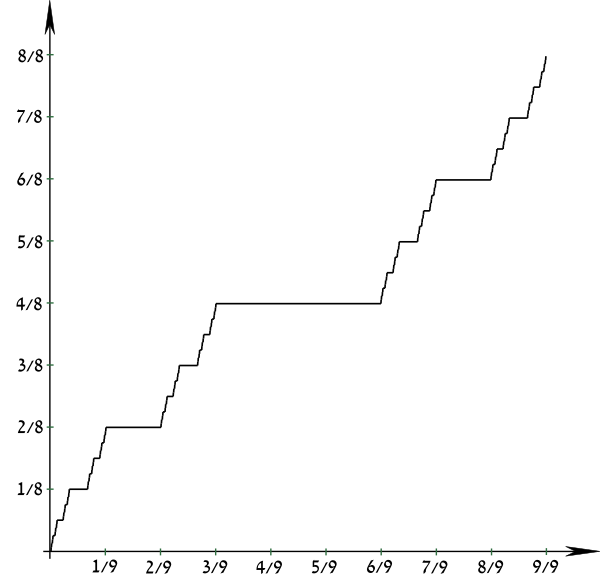
\includegraphics[scale=0.3]{img/devils_staircase.png}
      \caption{Plot} 
      \label{fig:devils_staircase}
    \end{figure}
  \end{definition} 

  \begin{theorem}
    $\phi$ is a nondecreasing, continuous function s.t. $\phi^\prime (x) = 0$ for all $x \in O$ and $m(O) = 1$. 
  \end{theorem}
  \begin{proof}
    Listed. 
    \begin{enumerate}
      \item \textit{Increasing}. $\phi$ is increasing on each $O_k$, and so on $O$. Then, it is also increasing on $C$ by definition. 
      \item \textit{Continuity}. If $x \in C$, it lies between 2 intervals of $O_k$ for any $k$. The difference in function values between 2 neighboring intervals of $O_k$ is $2^{-k}$, so $\phi$ is continuous. 
      \item \textit{Derivative}. The derivative is $0$ because it is constant around an interval. 
    \end{enumerate}
  \end{proof}

  \begin{theorem}[]
    Define $\psi (x) = \phi(x) + x$. Then, 
    \begin{enumerate}
      \item $\psi$ is continuous and strictly increasing. 
      \item $\psi$ maps $C$ into a set of positive measure. 
      \item $\psi$ maps some subset of $C$ into a nonmeasurable set. 
    \end{enumerate}
  \end{theorem}
  \begin{proof}
    Listed. 
    \begin{enumerate}
      \item Continuity is from sum of continuous functions, and strictly increasing since $\phi$ is nondecreasing and $x$ is strictly increasing. 
      \item We know that $\psi([0, 1]) = [0, 2]$ and $m(\psi(O))= 1$, where for each interval $I_j \subset O$, $m(\psi(I_j)) = \ell(I_j)$. Therefore, $m(\psi(C)) = 1$. 
      \item Since $\psi$ is strictly increasing, there exists a continuous inverse $\psi^{-1}$. Find $Z \subset \psi(C)$ that is nonmeasurable, which we can do from the previous theorem. Then, there exists $E \subset C$ s.t. $\psi(E) = Z$, and $E$ is not Borel since if it were, then $Z$ would be Borel, too. 
    \end{enumerate}
  \end{proof}

